\documentclass[crop,tikz]{standalone}
\usepackage[subpreambles=true]{standalone}

\input{preamble}

\begin{document}

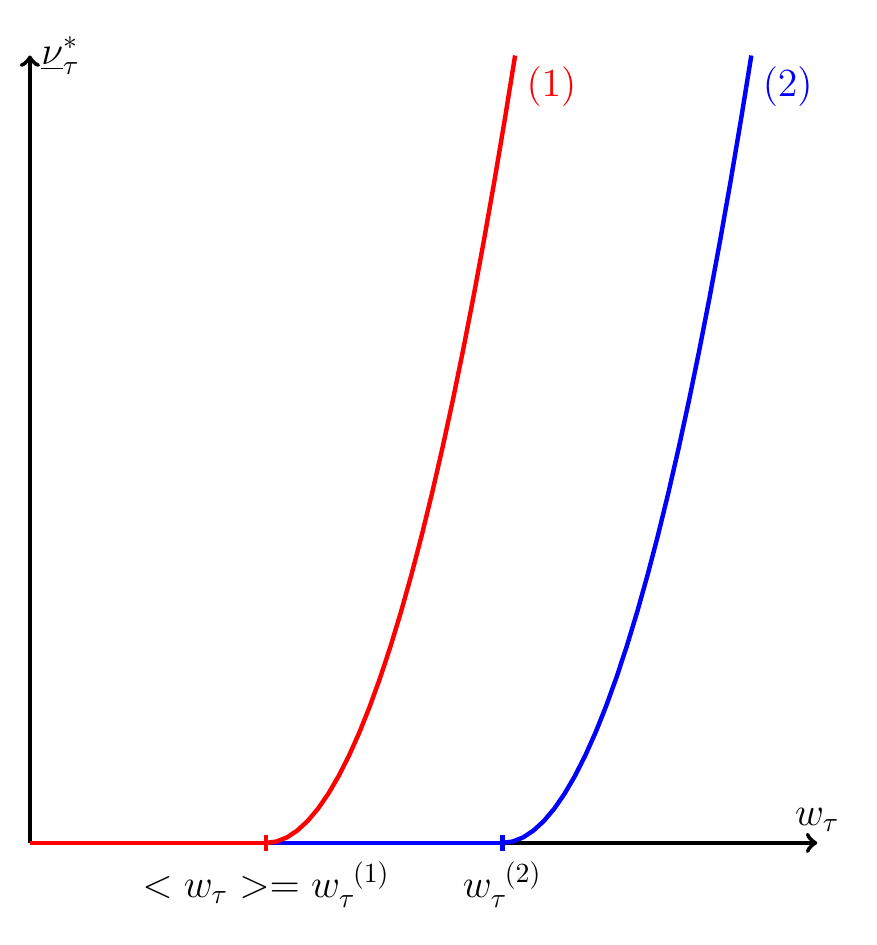
\begin{tikzpicture}[scale=1]

% axes
\draw[ultra thick] (0, 0)[->] -- (0, 10) node[right]{\Large $\underline{\nu}_{\tau}^*$};
\draw[ultra thick] (0, 0)[->] -- (10, 0) node[above]{\Large $w_{\tau}$};

% 1st line
\draw[ultra thick, blue] (0, 0) -- (6, 0);
\draw[ultra thick, blue] [domain=6:6+sqrt(10)] plot(\x,{(\x-6)^2}) node[below right]{\Large $(2)$};
% 2nd line
\draw[ultra thick, red] (0, 0) -- (3, 0);
\draw[ultra thick, red] [domain=3:3+sqrt(10)] plot(\x,{(\x-3)^2}) node[below right]{\Large $(1)$};

% ticks
\draw[red, ultra thick] (3, -0.1) node[below, black]{\Large $<w_{\tau}> = w_{\tau}^{~(1)}$} -- (3, 0.1);
\draw[blue, ultra thick] (6, -0.1) node[below, black]{\Large $w_{\tau}^{~(2)}$} -- (6, 0.1);

\end{tikzpicture}

\end{document}
